%Signal Generator Module

\subsubsection{Overview}
\label{Signal Generator}
\index{Signal Generator}\index{utilities, Signal Generator}

\begin{figure}[h]
\begin{center}
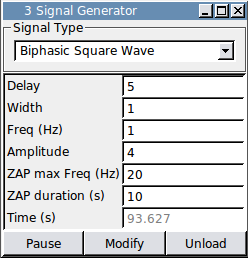
\includegraphics[width=2in]{siggen-tutorial1.png} 
\caption[Signal Generator]{The signal generator module is set to output a 1s long biphasic square wave every 5s, with an amplitude of 4. A tutorial is provided to replicate this figure.}
\end{center}
\label{siggen1}
\end{figure}

The signal generator module can generate a number of different signals, and each signal is modified through several parameters. The available signals and their corresponding parameters are described below.

\begin{itemize}
\item Sine Wave: requires frequency and amplitude
\item Monophasic Square Wave: requires delay, pulse width, and pulse amplitude
\item Biphasic Square Wave: requires delay, pulse width, and pulse amplitude
\item Sawtooth Wave: requires delay, pulse width, and maximum amplitude
\item ZAP Stimulus: needs starting and ending frequencies, amplitude, and duration of ZAP
\end{itemize}

All signals are continuous except for the ZAP stimulus, which has a specified duration.

\subsubsection{Output Channels}
\begin{description}
\item [Signal Waveform]Signal output
\end{description}

\subsubsection{Parameters}
\begin{description}
\item [Delay (s)]Time before each square wave or sawtooth wave starts
\item [Width (s)]Width of each square wave and sawtooth signal
\item [Freq (Hz)]frequency of sine wave and starting frequency for ZAP stimulus
\item [Amplitude]amplitude for all signals
\item [ZAP max Freq (Hz)]maximum frequency for ZAP stimulus
\item [ZAP duration (s)]duration of ZAP stimulus
\end{description}

\subsubsection{Tutorial}
\label{siggen tutorial}\index{Signal Generator, tutorial}\index{tutorial, Signal Generator}
In this tutorial, the Signal Generator will be used to output a biphasic square wave every 5s. Each phase will be 1s long, with an amplitude of 4. The oscilloscope will be used to visualize the signal, with the option of outputting the signal through a data acquisition board. The mimic tutorial continues where this tutorial leaves off,\seealso{Chapter \ref{mimic tutorial}\\Mimic Tutorial} so it is suggested that is done next.

\begin{enumerate}
\item Open the Signal Generator module through the menu: \textbf{Utilities}$\rightarrow$\textbf{Signals}$\rightarrow$\textbf{Signal Generator}
\item Open the oscilloscope module through the menu: \textbf{System}$\rightarrow$\seealso{Chapter \ref{Oscilloscope}\\Oscilloscope}\textbf{Oscilloscope}
\item Set the correct parameters for the desired biphasic square wave in the signal generator GUI as in Figure \ref{siggen1}:
  \begin{itemize}
  \item Set the signal type to \textbf{Biphasic Square Wave} using the pull down menu under \textbf{Signal Type}
  \item To output the signal every 5s, set \textbf{Delay} to 5
  \item To set each phase to be 1s long, set \textbf{Width} to 1
  \item To set the amplitude to 4V, set \textbf{Amplitude} to 4
  \item Save changes by clicking the \textbf{Modify} button
  \end{itemize}
\item Set up the oscilloscope to visualize the signal by right clicking on the oscilloscope and selecting \textbf{Properties}
  \begin{itemize}
  \item Make sure the \textbf{Channel} Tab is currently selected
  \item Select \textbf{Signal Generator} under the channel pulldown menu (This probably will already be selected)
  \item Select \textbf{Output} in the following pulldown menu on the right
  \item Select \textbf{Signal Waveform} in the following pulldown menu on the right (This probably will already be selected)
  \item Activate this channel by hitting the toggle button \textbf{Active}
  \item Change the scale to \textbf{1 V/div} in the Scale pulldown menu
  \item Click the \textbf{Apply} button to save the changes
  \item Select the \textbf{Display} tab
  \item Change the time scale to \textbf{1 s/div}
  \item Change the refresh rate to 50 for a smoother looking output
  \item Click the \textbf{Apply} button to save the changes
  \end{itemize}
\item \textit{Optional} Output the signal generator signal through the analog output of a data acquisition board
  \begin{itemize}
  \item Open the connector module through the menu: \textbf{System}$\rightarrow$\textbf{Connector}
  \item In the Output Block, select \textbf{Signal Generator} under block and \textbf{Signal Waveform} under Channel
  \item In the Input Block, select your data acquisition board (i.e. /dev/comedi0 or NI-PCI6259) and the desired channel (i.e. Analog Output 0)
  \item Connect the two by toggling the arrow button
  \item Make sure the desired channel is active through the \seealso{Chapter \ref{system control panel}\\System Control Panel}System Control Panel
  \end{itemize}
\item Start the signal by untoggling the \textbf{Pause} button
\item The biphasic square wave should now be seen on the oscilloscope as in Figure \ref{siggen1}
\end{enumerate}

\begin{figure}[h]
\begin{center}
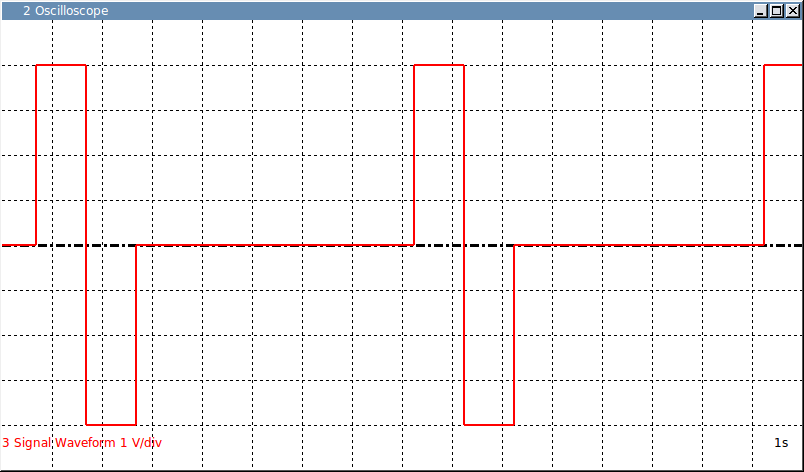
\includegraphics[width=4.5in]{siggen-tutorial2.png} 
\caption[Signal Generator Output]{The oscilloscope is used to visualize a biphasic square wave being output by the Signal Generator Module} 
\end{center}
\label{siggen2}
\end{figure}